\chapter{TTSP Implementation}

%-----------------------------------------------------------
% keywords: Reference implementation
%-----------------------------------------------------------
As previously said, a reference implementation was also developed. This intention had the purpose of demonstrating that such architecture could be implemented but also to validate and evaluate its effectiveness and efficiency that can be achieved with it. This reference implementation was developed on the Crossbow MICAz hardware platform which executed the TinyOS platform, which is mainly described for being very low resource demanding and having an event-centric and a modular component architecture. TTSP was implemented as a TinyOS library, thus, it is made available to every other component of the operating system (including the already available MAC protocols) and the upper lying TinyOS application developed by the user. 

\setcounter{secnumdepth}{2}
\section{Development hardware and software platform}
%-----------------------------------------------------------
% keywords: Development hardware and software platform
%-----------------------------------------------------------

\subsection{Hardware platform}
%-----------------------------------------------------------
% keywords: Crossbow MICAz 
%-----------------------------------------------------------
TTSP reference implementation has been developed on the TinyOS 2.x software platform, and has been primarily tested on Crossbow MICAz sensor nodes \cite{crossbow04}. The Crossbow MICAz is a commercially available sensor platform that couples an 8-bit AVR RISC microcontroller, the Atmel ATmega128L \cite{atmel08}, with an IEEE 802.15.14 Zigbee-ready transceiver, the Chipconn CC2420 \cite{cc04}. The use of this platforms, in itself, is a challenge to overcome, especially due to the reduced amount of available memory on the MICAz sensor node (4 kB of SRAM).\\
The relatively limited amount of memory on this type of hardware platform posed some implementation challenges to the developer. One most take into account that the developed TTSP library will eventually be used in conjunction with an application, so in order not to limit even more the development of applications regarding memory size, developed libraries must try to squeeze its size to the maximum.\\
As we will see next, most of the software code developed over this platform has been re-factorized in order to guarantee its minimum implementation footprint.

\subsection{Software platform}
%-----------------------------------------------------------
% keywords: Monolothic architecture
%-----------------------------------------------------------
TinyOS, is an open-source operating system initially developed at the University of California, Berkeley. This operating system was specifically designed to work on embedded systems with very severe computational constraints, such as those found in WSNs, and has, since then, become the de facto standard operating system for several WSN platforms.\\
TinyOS combines flexible, fine-grain components with an execution model that supports complex yet safe concurrent
operations. Its built from a set of reusable components that are assembled into an application-specific system. Like the
applications, the solution is event-centric. The normal operation is the reactive execution of concurrent events. This event-driven concurrency model is based on split-phase interfaces, asynchronous events, and deferred computation called tasks.
These component and execution models avoid the use of complex structures for scheduling and locking mechanisms between
tasks lowering the need for memory resources.\\
This specialized architecture is further supported by a specialized C-like programming language, with which all TinyOS components must be programmed, called nesC \cite{gay03}. The application is statically linked with the kernel to create a
complete image of the system at compile-time. After linking, modifying the system is not possible.

\begin{itemize}
\item Limited resources
\item Flexibility
\item Concurrency
\item Power management
\end{itemize}

The module of construction of TinyOS is built around these four main goals and it encompasses all the general features that
are expected of a sensor node operating system to perform effectively and also maximize performance.
Additionally, TinyOS provides a powerful simulation environment, TOSSIM \cite{levis03} \cite{lee03}, which enables the simulation of entire WSNs using the same source-code that is used on real sensors.

\section{Implementation considerations and complexity}
%-----------------------------------------------------------
% keywords: Implementation details and complexity
%-----------------------------------------------------------
As previously said, TTSP was implemented as a library that can be included and used by any application. Its implementation follows a modular approach, in which, each of the three principles of synchronization logic used by TTSP are encapsulated in their own modules. This modular approach eases software development and its debugging. Additionally, as already stated here, it allows one to easily switch or modify the corresponding synchronization logic without breaking the remaining other logic blocks. The complexity aimed for TTSP's implementation development was to be minimal as possible. The chosen synchronization techniques are easily implemented and its simple behaviour (yet theoretical efficient) facilitates debugging.

\subsection{Implementation considerations}
%-----------------------------------------------------------
% keywords:
%-----------------------------------------------------------
Although the implementation of TTSP did not pose serious constraints to the proposed conceptual architecture, there are some important considerations to retain from this process, especially those that have a great impact on the overall performance of TTSP in real-life scenarios, whether it be the interfaces that the common developer will need to master in order to make their applications and MAC protocols aware of TTSP services or the synchronization period adjustment algorithm which is the core piece of TTSP and may be tunable/hackable in order to satisfy exquisite network topologies. Additionally, some implementation considerations are needed for non-trivial synchronization techniques.

\subsubsection{Interfaces}
%-----------------------------------------------------------
% keywords:
%-----------------------------------------------------------
Regarding the interfaces that are available to interact with TTSP, the most important one is AdaptiveTimeSync. This interface is exported to the application and MAC-layer protocol. The signature of the AdaptiveTimeSync interface is depicted in Figure \ref{adapttimeysnc}. This interface tells us that the clients of TTSP should implement both the synchronized and unsynchronized events while TTSP should implement all the remaining commands that are to be used.

\begin{figure}[!htb]
\begin{center}
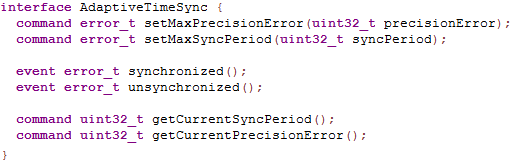
\includegraphics[scale=0.5]{./images/27-ttsp-code_interfaces.png}
\end{center}
\caption{AdaptiveTimeSync interface.}
\label{adapttimeysnc}
\end{figure}

As explained in the previous chapter, these interfaces are exported by the adaptive synchronization logic implementation. With regard to memory constraints (in this case heap memory size) and number of CPU instructions, the remaining interfaces are exported from the pair-wise and network-wide synchronization logic modules. This avoids unnecessary memory usage and increases the execution speed overall of the following commands.\\
The following interface that is exported to the application layer and MAC-layer is a more simpler to use but still deeply important, as it allows the application or the MAC-layer protocol to be aware of the logical clock. This interface can be found in Figure \ref{globaltime}.

\begin{figure}[!htb]
\begin{center}
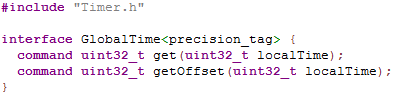
\includegraphics[scale=0.5]{./images/28-ttsp-code_interfaces2.png}
\end{center}
\caption{GlobalTime interface.}
\label{globaltime}
\end{figure}

The last remaining interface that can be seen in Figure \ref{timesyncinfo} allows the application to get some knowledge whether it is the root or if not, the root node to which the node is synchronized.

\begin{figure}[!htb]
\begin{center}
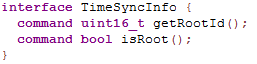
\includegraphics[scale=0.5]{./images/29-ttsp-code_interfaces3.png}
\end{center}
\caption{TimeSyncInfo interface.}
\label{timesyncinfo}
\end{figure}

An overall view of the wiring of the AdaptiveTimeSyncP and its components and interfaces can be viewed in Figure \ref{compwiring}.

\begin{figure}[!htb]
\begin{center}
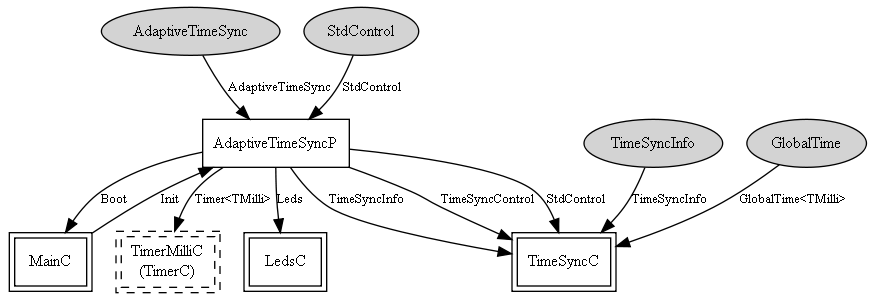
\includegraphics[scale=0.4]{./images/30-ttsp-interface_wiring.png}
\end{center}
\caption{Wiring of AdaptiveTimeSyncP component and its application and MAC-layer interfaces.}
\label{compwiring}
\end{figure}

On the other side, we have another special interface which interacts between the AdaptiveTimeSyncP component and the pair-wise and network-wide synchronization logic (which is encapsulated in TimeSyncP component), the TimeSyncControl interface. This special and more complex interface is the glue between the adaptive time synchronization and the pair-wise and network-wide synchronization. This interface exports control of the underlying mechanisms for pair-wise and network-wide synchronization to the adaptive time synchronization logic component. The Figure \ref{timesynccontrol} shows an excerpt of the commands and events that this interface exports.

\begin{figure}[!htb]
\begin{center}
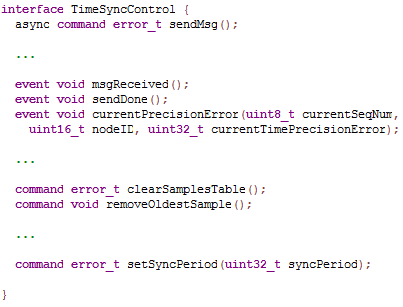
\includegraphics[scale=0.5]{./images/36-ttsp-code_interfaces4.png}
\end{center}
\caption{TimeSyncControl interface.}
\label{timesynccontrol}
\end{figure}

Finally, an overview of the wiring of the TimeSyncP and its components and interfaces can be viewed in Figure \ref{timecomp}.

\begin{figure}[!htb]
\begin{center}
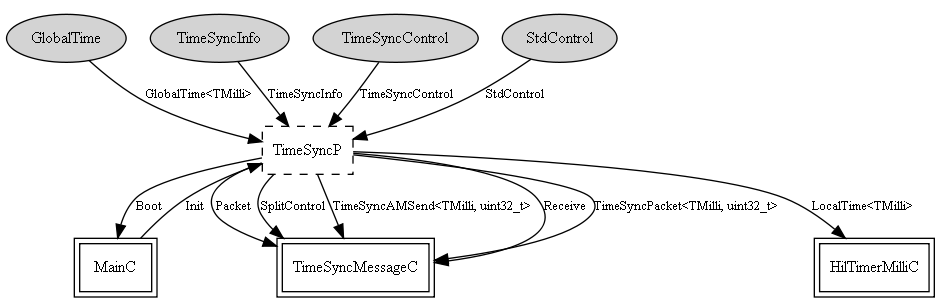
\includegraphics[scale=0.4]{./images/35-ttsp-interface_wiring2.png}
\end{center}
\caption{Wiring of TimeSyncP component and its interfaces.}
\label{timewiring}
\end{figure}

\subsubsection{MAC-layer time-stamping}
%-----------------------------------------------------------
% keywords:
%-----------------------------------------------------------
Typically, in TinyOS neither the time of invocation of the send command, nor the time of signalling of the sendDone event can be used to estimate, without significant jitter, the time when the packet was transmitted. Similarly, the time of occurrence of the receive event cannot be used to reliably estimate the time of reception. A straightforward way of message time-stamping while reducing the delay uncertainty, is to place these time-stamps when the message is being sent at the MAC-layer. TinyOS exposes a specialized interface which allows one to send messages while placing a time-stamp at the MAC-layer. Typically, this interface makes use of the \ac{SFD} interrupt handler on the CC2420 radio, which allows TinyOS to know when to place the time-stamp while sending the message through the radio.

The TimeSyncAMSend interface allows one for sending this time-stamp along with a message. This interface can be seen in Figure \ref{timesyncamsend}.

\begin{figure}[!htb]
\begin{center}
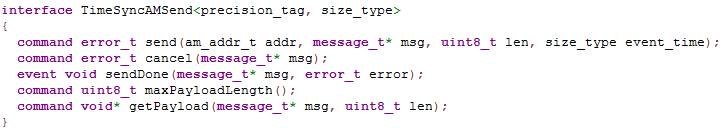
\includegraphics[scale=0.5]{./images/31-ttsp-mac_timestamp.png}
\end{center}
\caption{TimeSyncAMSend interface used for placing time-stamps on outgoing messages.}
\label{timesyncamsend}
\end{figure}

On the opposite side, that is on the receiving side, one can use the TimeSyncPacket interface to retrieve the time-stamp of the message. This interface is depicted in Figure \ref{timesyncpacket}.

\begin{figure}[!htb]
\begin{center}
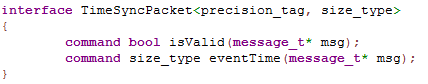
\includegraphics[scale=0.5]{./images/32-ttsp-mac_timestamp2.png}
\end{center}
\caption{TimeSyncPacket interface used for retrieving the time-stamp sent along with the received packet.}
\label{timesyncpacket}
\end{figure}
 
For example, when TTSP uses the TimeSyncAMSend.send command called with event time-stamp t1, it stores t1 and sends the packet to the MAC-layer. When the packet starts being transmitted over the communication medium, a corresponding hardware event is timestamped (an SFD interrupt). Let us denote this transmission time-stamp with t2. The difference of event time-stamp t1 and transmit time-stamp t2 is written into the designated time-stamp field in the payload of the packet (typically into the footer, since the first few bytes might have been transmitted by this time). That is, the information the packet contains at the instance when being sent over the communications medium is the age of the event (i.e. how much time ago the event had occurred).\\
In the receiver side, when the packet is received, it is timestamped with the receiver node's local clock at reception (e.g. with the time-stamp of the SFD interrupt). Let us denote the time of reception with t3. When the event time is queried via the TimeSyncPacket interface, the eventTime command returns the sum of the value stored in the designated time-stamp field in packet payload and the reception time-stamp, i.e. t1- t2+t3. This value corresponds to the time of the event in the receiver's local clock.

%\subsubsection{Skew compensation mechanism}%

\subsubsection{Synchronization period adjustment algorithm}
%-----------------------------------------------------------
% keywords:
%-----------------------------------------------------------
As previously said, the core piece of the adaptive approach of TTSP, is its synchronization period adjustment algorithm. This algorithm already has been explained in the previous chapter. The implementation of this algorithm was rather trivial, since it was modelled to be a finite-state machine. Implementing finite-state machine is accomplished by saving the current state and typically using a switch code block.\\
The Figure \ref{adaptivecode} depicts a code excerpt of the switch code block that implements the phase 1 of synchronization period adjustment finite-state machine.

\begin{figure}[!htb]
\begin{center}
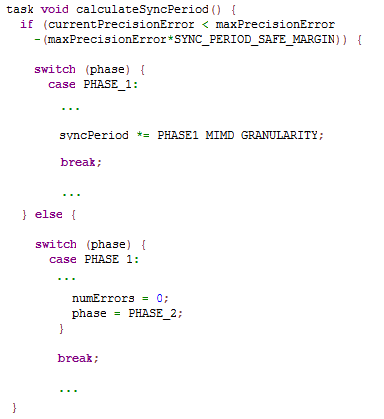
\includegraphics[scale=0.5]{./images/33-ttsp-adaptive_code.png}
\end{center}
\caption{Code excerpt of the switch code blocks used to implement phase 1 of the finite-state machine.}
\label{adaptivecode}
\end{figure}

The previous code block is executed whenever the root node has some feedback of the time precision of its neighbours. That is, when the pair-wise and network-wide synchronization components signal through an event the adaptive synchronization module. Thus, the code used for adjusting the synchronization period was placed on an individual task, due to the fact that its execution could starve other event signal flows in the operating system.

Once a new synchronization period is obtained, it is ready to be broadcasted by the root to the neighbouring nodes. In order to rapidly apply and start broadcasting the new synchronization period, the next synchronization round will be also recalculated in order to compensate those cases when the new synchronization period is less than the previous. The code developed for the described function is depicted in Figure \ref{adaptivecode2}.

\begin{figure}[!htb]
\begin{center}
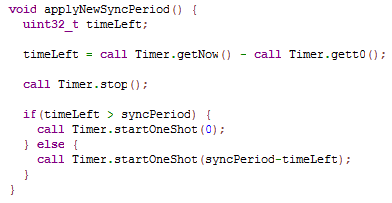
\includegraphics[scale=0.5]{./images/34-ttsp-adaptive_code2.png}
\end{center}
\caption{Code of the function to rapidly apply the new synchronization period.}
\label{adaptivecode2}
\end{figure}

\subsection{Implementation complexity}
%-----------------------------------------------------------
% keywords: Implementation complexity
%-----------------------------------------------------------
One of the goals set for TTSP was its ease of implementation, and verifying it was also one of the reasons leading to the development of this prototype. While ease of implementation is always a topic of subjective evaluation, some objective metrics can be presented.\\
The full implementation contains 10 components (configurations, modules and interfaces) and 1039 physical source lines of code (SLOC), excluding utilities and debugging functionality.
Regarding memory usage, an image ready to be flashed on a node compiled with a dummy application and TTSP, occupies 1903 bytes of RAM and 22487 bytes of ROM. So to speak, that leaves plenty of memory (both types) for the application developer.

\section{Redesign of Tagus-SensorNet}
%-----------------------------------------------------------
% keywords: Redesign of Tagus-SensorNet
%-----------------------------------------------------------
Regarding the test-bed itself and in parallel with TTSP development, there was an effort in redesigning Tagus-SensorNet to become more flexible in handling multiple and both software and hardware heterogeneous WSN's islands under one single software application development platform. The need came from the fact that multiple independent and many times strictly communication closed WSN's islands were starting to appear in Tagus-SensorNet (as a result of the increasing scientific interest that WSN is having at the moment). The previous architecture was unable to allow these new islands to communicate between themselves, the need to have multiple base-stations (sink nodes), each WSN island required its own base-station, but also do to the application development that much of the time was repeating already existent source code. This need led to propose a new architecture for Tagus-SensorNet which would also ease TTSP during its evaluation phase.

\subsection{Previous Tagus-SensorNet architecture}
%-----------------------------------------------------------
% keywords: Monolothic architecture
%-----------------------------------------------------------
Until recently, Tagus-SensorNet architecture had a monolithic structure which clearly was designed taking into account the limited set of hardware platforms commercially available at that time, the most popular operating system (TinyOS) and by that extent the limited number of available MAC-layer and network layer protocols. This architecture clearly satisfied its initial needs, that was to allow the application developer to interact with the nodes in a given application. Using this architecture the application developer tended to develop specifically TinyOS code on the nodes tightly coupled with the application itself. As we later became aware, much of the code was being repeated over time. And worst, many times this application code was being developed specifically for a given hardware platform.\\
Also, with the growth of the network, multiple WSN islands were being deployed to test and bench-mark a variety of protocols. The previous architecture clearly failed to allow these new islands to communicate between themselves if by any means they used a different MAC-layer protocol or a different radio frequency.

\subsection{Proposed and implemented changes}
%-----------------------------------------------------------
% keywords: 
%-----------------------------------------------------------
The proposed architecture decouples the embedded software running on the nodes hardware platform and the application itself. This way, it is possible to allow hardware and software heterogeneity in the network without implementing a MAC-layer or network layer protocol that is common on every node. This clearly makes way to a inter-networking between nodes, WSNs and applications made at the application layer. The proposed architecture can be seen in Figure \ref{tsnng}.

\begin{figure}[!htb]
\begin{center}
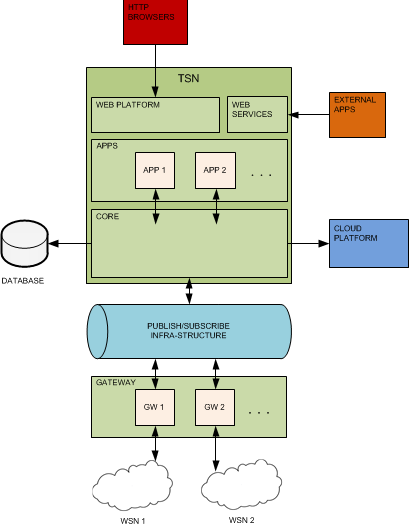
\includegraphics[scale=0.5]{./images/37-ttsp-tsn_ng.png}
\end{center}
\caption{Tagus-SensorNet proposed architecture.}
\label{tsnng}
\end{figure}

The major contribution with this design is made by the publish/subscribe infra-structure which is able to support multiple communication flows through message label multiplexing, this offers extremely flexibility on the way applications interact with different WSNs and eventually nodes. Applications publish messages to specific WSN islands and nodes. On the other end gateways subscribe to those messages and convert the message to the specific network protocol being executed at that WSN island and vice-versa.\\
This new architecture clearly enables a new paradigm of WSN application development flexibility and interaction. Other components were thought to be added in a future stage, such as interface with a cloud computing platform, export a Web Services API to allow other ways of interfacing with Tagus-SensorNet and GUI related interfaces. With this said, Tagus-SensorNet architecture changes ease application development and interaction with the WSN, which eventually facilitated TTSP development and evaluation.\\

A global overview of f TTSP implementation considerations as also other related work was given throughout this chapter. It is worth to mention that TTSP’s reference implementation has been freely contributed to TinyOS contributions repository under the GEMS group directory.